\documentclass{article}

% Default packages
\usepackage[utf8]{inputenc}
\usepackage[spanish]{babel}
\usepackage{fancyhdr}
\usepackage{tikz}
\usepackage{amssymb}

\usepackage{listings}
\usepackage{xcolor}

\lstset{
    showstringspaces=false, % don't mark spaces in strings
    numbers=left, % display line numbers on the left
    commentstyle=\color{blue}, % comment color
    keywordstyle=\color{magenta}, % keyword color
    stringstyle=\color{red} % string color
}

\usepackage{graphicx}
\graphicspath{ {./imagenes/} }

\usepackage{geometry}
\geometry{margin=2cm}

\title{Sigma}
\author{Axel Treviño Palacios} 
\date{31 de Octubre de 2020}
\def\thenumber{1}

\makeatletter
\let\thetitle\@title
\let\theauthor\@author
\let\thedate\@date
\makeatother

\pagestyle{fancy}
\fancyhead{}
\fancyfoot{}
\fancyfoot[R]{\thepage}
\fancyfoot[L]{\thetitle}
\renewcommand{\headrulewidth}{0pt}
\renewcommand{\footrulewidth}{0.5pt}

\begin{document}
	\begin{titlepage}
		\centering	 
	 	
	 	\begin{tikzpicture}[remember picture, overlay]
			\node[anchor=north east,inner sep=1cm] at (current page.north east)
				{
\includegraphics[height=3.5cm]{logoEscom}};
			\node[anchor=north west,inner sep=1cm] at (current page.north west)
				{
\includegraphics[height=3.5cm]{logoPoli}};
		\end{tikzpicture}

		\vspace{4cm}
		{\Large \scshape Instituto Politécnico Nacional \par}
		\vspace{1cm}

		{\rmfamily \bfseries \Large Escuela Superior de Cómputo \par}
		\vspace{4cm}

		{\itshape\Large Práctica \#\thenumber \par}
		\vspace{0.5cm}
		
		{\scshape\Huge \thetitle \par}
		\vspace{5cm}
			
		{\itshape\Large \theauthor \par}
		2CM5
		
		\thedate				
		
		\vfill
	\end{titlepage}

	\section{Objetivo}
	Programar el universo de las cadenas binarias \( \Sigma^n \). Dada una 'n' que introduzca el usuario o que el programa lo determine automáticamente. El rango de 'n' debe de estar en el intervalo de [0,1000].
\begin{enumerate}
	\item  El programa debe de preguntar si quiere calcular otra 'n' o no.
	\item La salida, expresada en notación de conjunto, debe ir a un archivo de texto.
	\item Una segunda salida (archivo de texto) debe concatenar todas las cadenas calculadas en una sola cadena, quitar las llaves, comas y cualquier otro símbolo que no sean 0s y 1s.
	\item Del primer archivo de salida, graficar el número de 1s de cada cadena. El eje de las x es la cadena y el eje de las y el número de 1s que tiene esa cadena. Específicamente, calcular y graficar cuando n=23. Al mismo tiempo, calcular la gráfica pero calculando su logaritmo en base 2 y 10 respectivamente.
	\item Del segundo archivo de salida, particionar la cadena en subcadenas de longitud 32 y graficar la cantidad de unos de esas subcadenas. Al mismo tiempo, calcular la gráfica pero calculando su logaritmo en base 2 y 10 respectivamente.
\end{enumerate}
	
	\section{Codigo}
	\lstinputlisting[language=C++]{sigma.cpp}
	\section{Conclusiones}
	Las computadoras, aunque increíblemente potentes, aun necesitan de nuestra ayuda para no matarse a sí mismas.
	\section{Resultado}
		\centering
		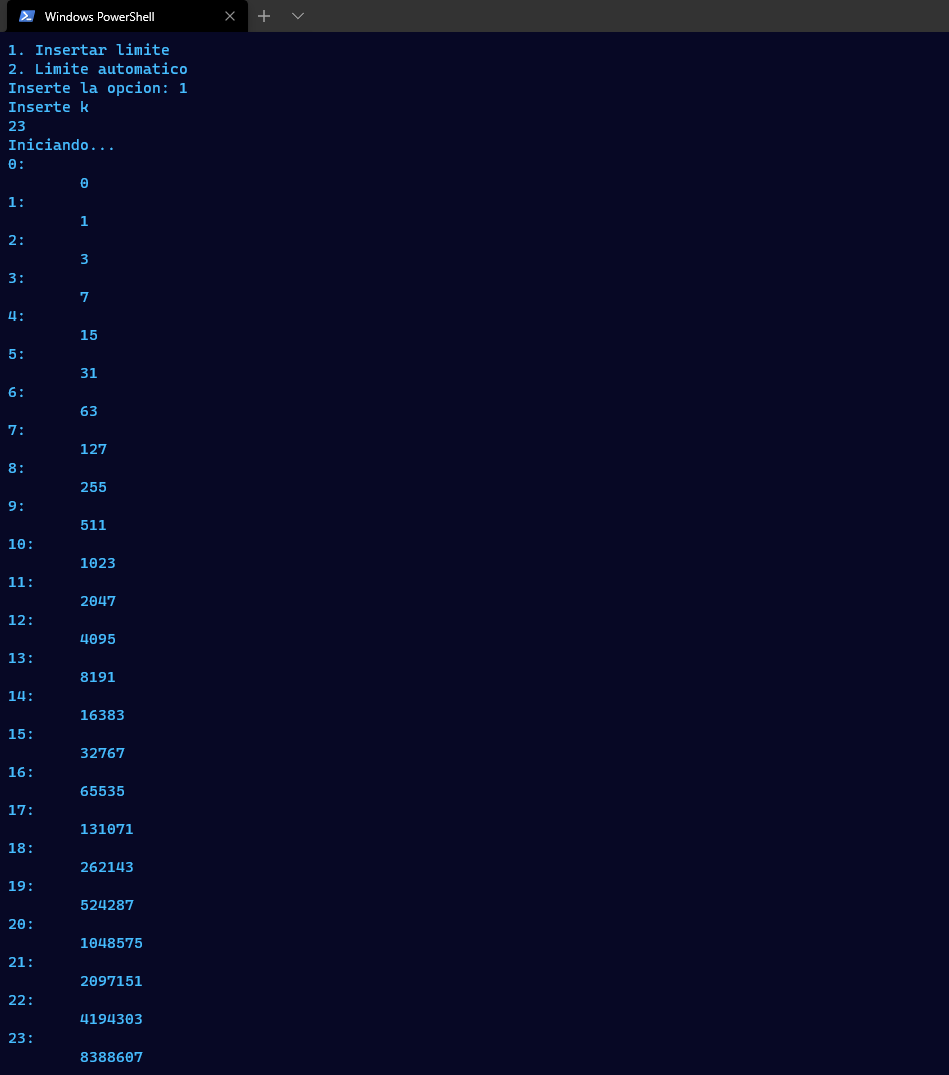
\includegraphics[height=0.8\textheight]{sigma1}
		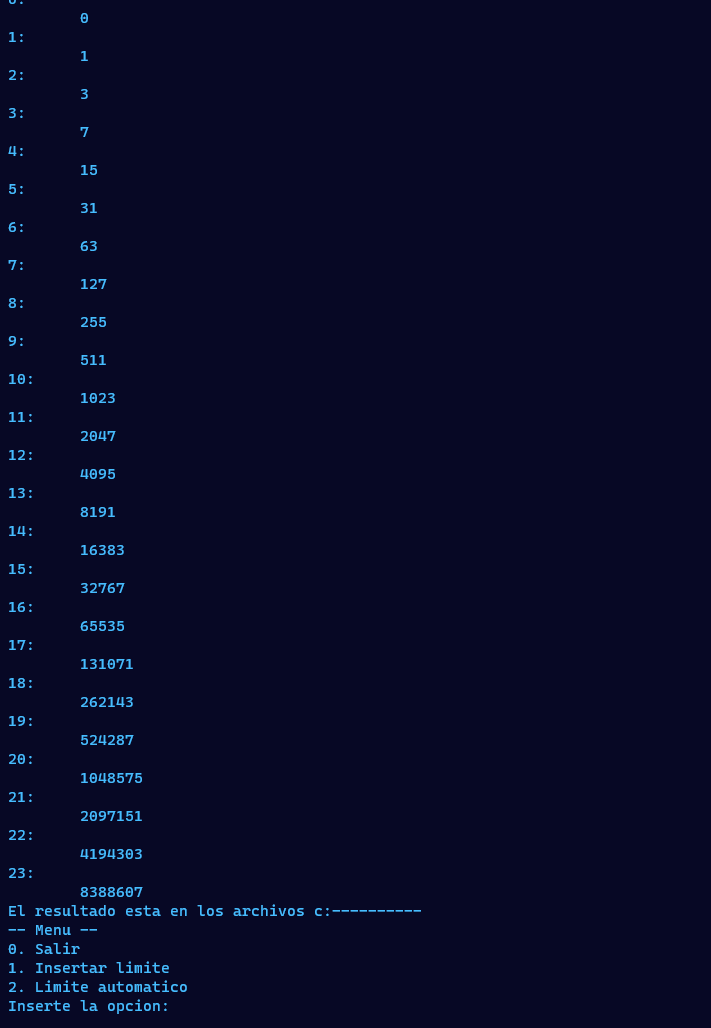
\includegraphics[height=\textheight]{sigma2}
		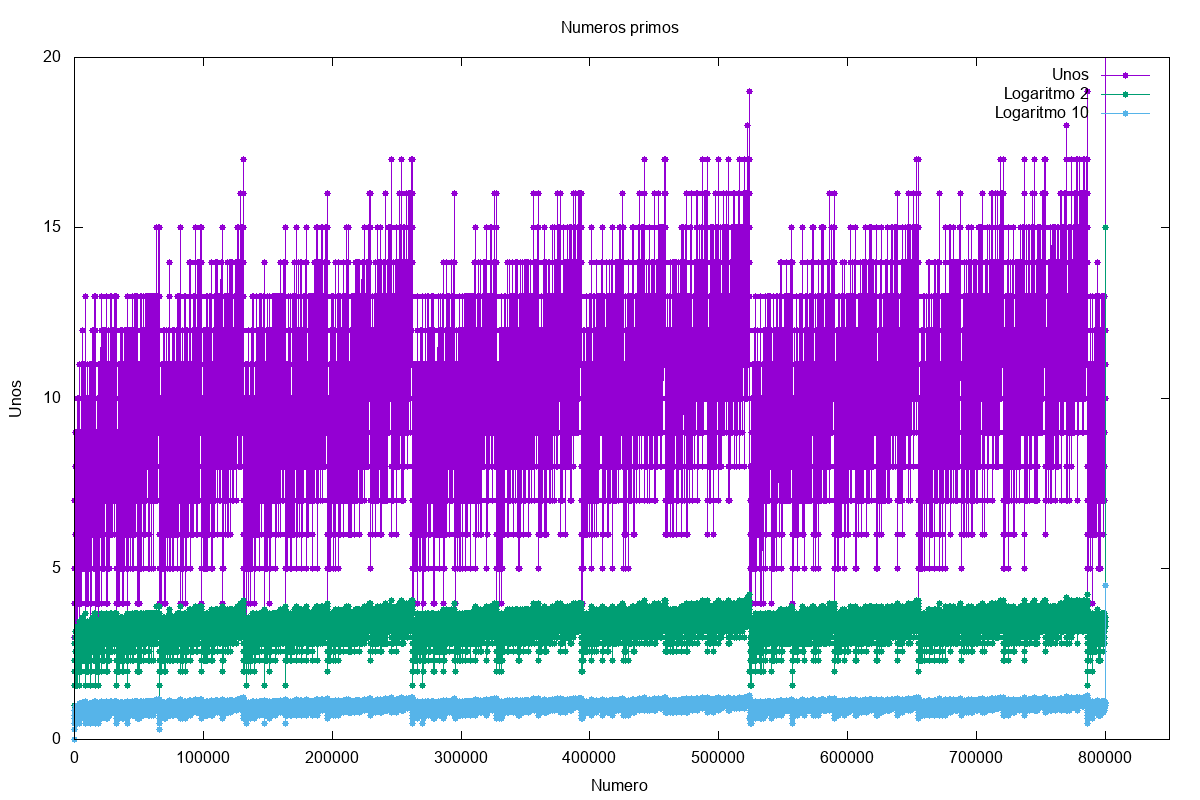
\includegraphics[width=\textwidth]{grafica}
		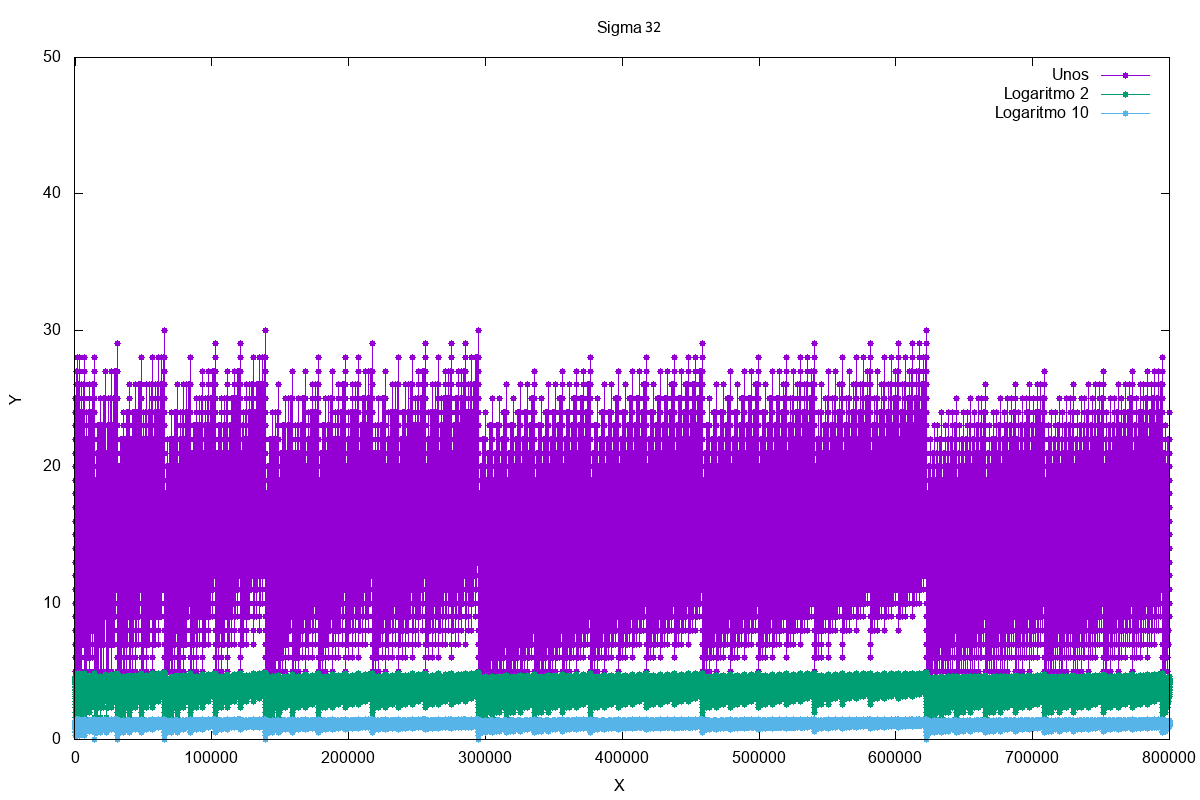
\includegraphics[width=\textwidth]{grafica32}

\end{document}